\documentclass{article}
\usepackage{iclr2026_conference,times}
\input{math_commands.tex}
\usepackage{hyperref}
\usepackage{url}
\usepackage{booktabs}
\usepackage{graphicx}

\title{Embodied Model Repair Memory: A Real MuJoCo Negative Result}
\author{Anonymous Authors}

\begin{document}
\maketitle

\begin{abstract}
The original hypothesis behind Embodied Model Repair Memory was that robots should store repairs to physical model beliefs as reusable state rather than treating corrections as transient prompts. We rebuild the idea as a real sequential MuJoCo benchmark with persistent hidden deployment shifts, implemented baselines, ablations, learning curves, and paired deltas. The result is negative. kNN residual repair memory does not beat nominal MPC or robust worst-case MPC, and simple global/last repair baselines are competitive or better in several regimes. This paper is therefore not an ICLR-main submission candidate. The honest terminal decision is \textbf{KILL\_ARCHIVE}. Submission-hardening version: v4.
\end{abstract}

\section{Motivation}
Long-horizon robot systems repeatedly encounter similar physical model errors: a surface is more slippery than expected, an actuator has a persistent gain error, or an obstacle is shifted relative to the nominal world model. A plausible repair-memory hypothesis is that the system should reuse previous embodied residuals when selecting future actions.

The v3 version of this paper was archived because it only had synthetic evidence. The v4 rebuild tests the hypothesis in a real MuJoCo sequential benchmark. The goal is not to rescue the paper rhetorically; it is to determine whether the mechanism survives a real evidence gate.

\section{Benchmark}
We use a planar MuJoCo contact-pushing task. A pusher moves a cylindrical puck toward a target while avoiding an obstacle. Each split/seed defines a persistent hidden deployment condition: mass, friction, actuation gain, angle bias, lateral bias, and obstacle shift remain fixed across a sequence of tasks. This creates recurring model error that a repair memory could exploit.

Each method sees the same deployment streams. The main run uses 5 seeds, 24 episodes per seed/split/method, and six stress splits: nominal, low-friction shift, high-friction shift, heavy-object shift, actuation-bias shift, and combined shift. The full run contains 5,040 main rows and 840 ablation rows.

\section{Methods}
The proposed embodied repair memory stores residuals between nominal predicted puck displacement and actual MuJoCo displacement. At the next task, it retrieves nearest residuals using action/geometry/context features and corrects nominal candidate rollouts before selecting an action.

Baselines are random candidate selection, nominal MPC, robust worst-case MPC, last-repair memory, global-average repair, and oracle hidden-deployment selection. Ablations reset memory every episode, remove context features, limit memory capacity, compare global repair, and compare nominal/oracle selectors.

\section{Main Results}
Table~\ref{tab:main} reports success rates. The proposed method improves over random but fails the decisive-baseline test. It loses to or ties nominal MPC on all splits, loses to robust MPC on most splits, and is not consistently better than global or last repair.

\begin{table}[t]
\centering
\caption{Success rate by stress split. Each entry is mean $\pm$ 95 percent CI over 120 episodes.}
\label{tab:main}
\small
\begin{tabular}{lccccc}
\toprule
Split & Repair memory & Nominal & Robust & Global repair & Oracle \\
\midrule
Nominal & $0.225 \pm 0.075$ & $0.242 \pm 0.077$ & $0.242 \pm 0.077$ & $0.250 \pm 0.078$ & $0.325 \pm 0.084$ \\
Low friction & $0.058 \pm 0.042$ & $0.058 \pm 0.042$ & $0.058 \pm 0.042$ & $0.058 \pm 0.042$ & $0.158 \pm 0.066$ \\
High friction & $0.142 \pm 0.063$ & $0.200 \pm 0.072$ & $0.208 \pm 0.073$ & $0.225 \pm 0.075$ & $0.383 \pm 0.087$ \\
Heavy object & $0.175 \pm 0.068$ & $0.192 \pm 0.071$ & $0.200 \pm 0.072$ & $0.192 \pm 0.071$ & $0.408 \pm 0.088$ \\
Actuation bias & $0.217 \pm 0.074$ & $0.242 \pm 0.077$ & $0.233 \pm 0.076$ & $0.217 \pm 0.074$ & $0.417 \pm 0.089$ \\
Combined shift & $0.117 \pm 0.058$ & $0.158 \pm 0.066$ & $0.150 \pm 0.064$ & $0.150 \pm 0.064$ & $0.258 \pm 0.079$ \\
\bottomrule
\end{tabular}
\end{table}

\begin{figure}[t]
\centering
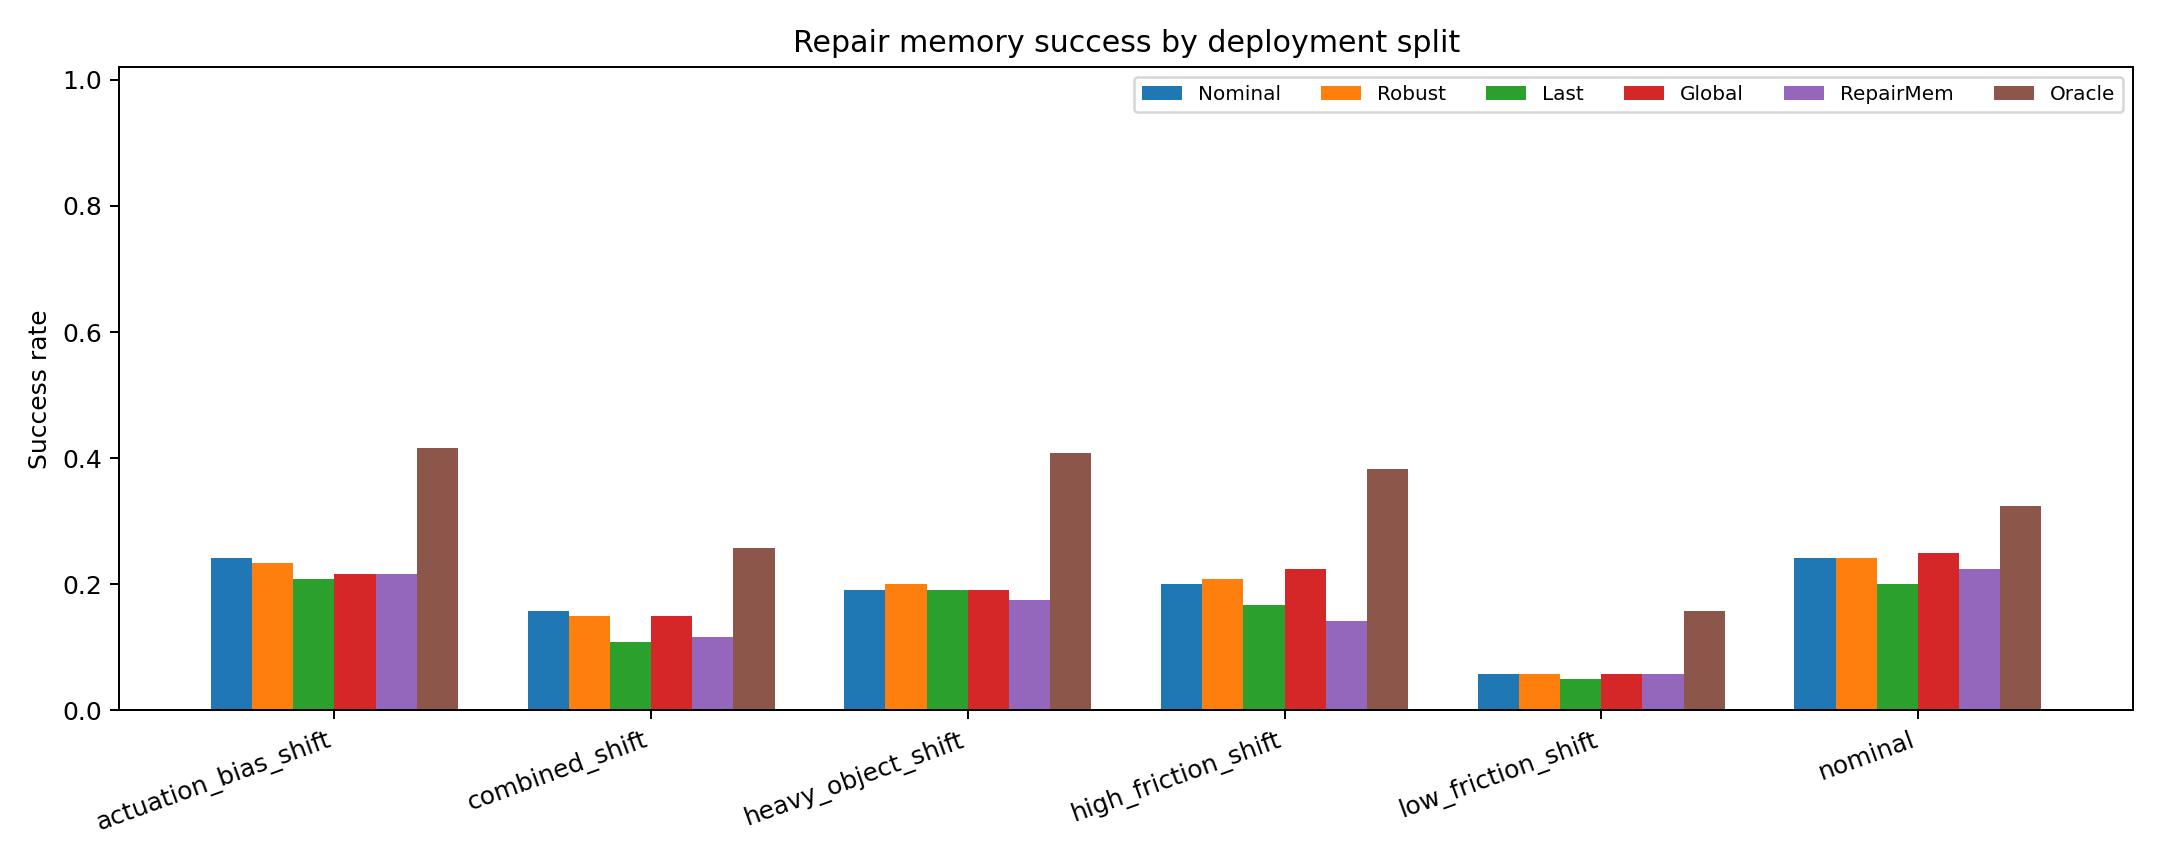
\includegraphics[width=\linewidth]{../figures/repair_success_by_split.png}
\caption{Repair-memory success rates across deployment shifts. The proposed method does not separate from nominal, robust, or simple repair baselines.}
\label{fig:success}
\end{figure}

\begin{figure}[t]
\centering
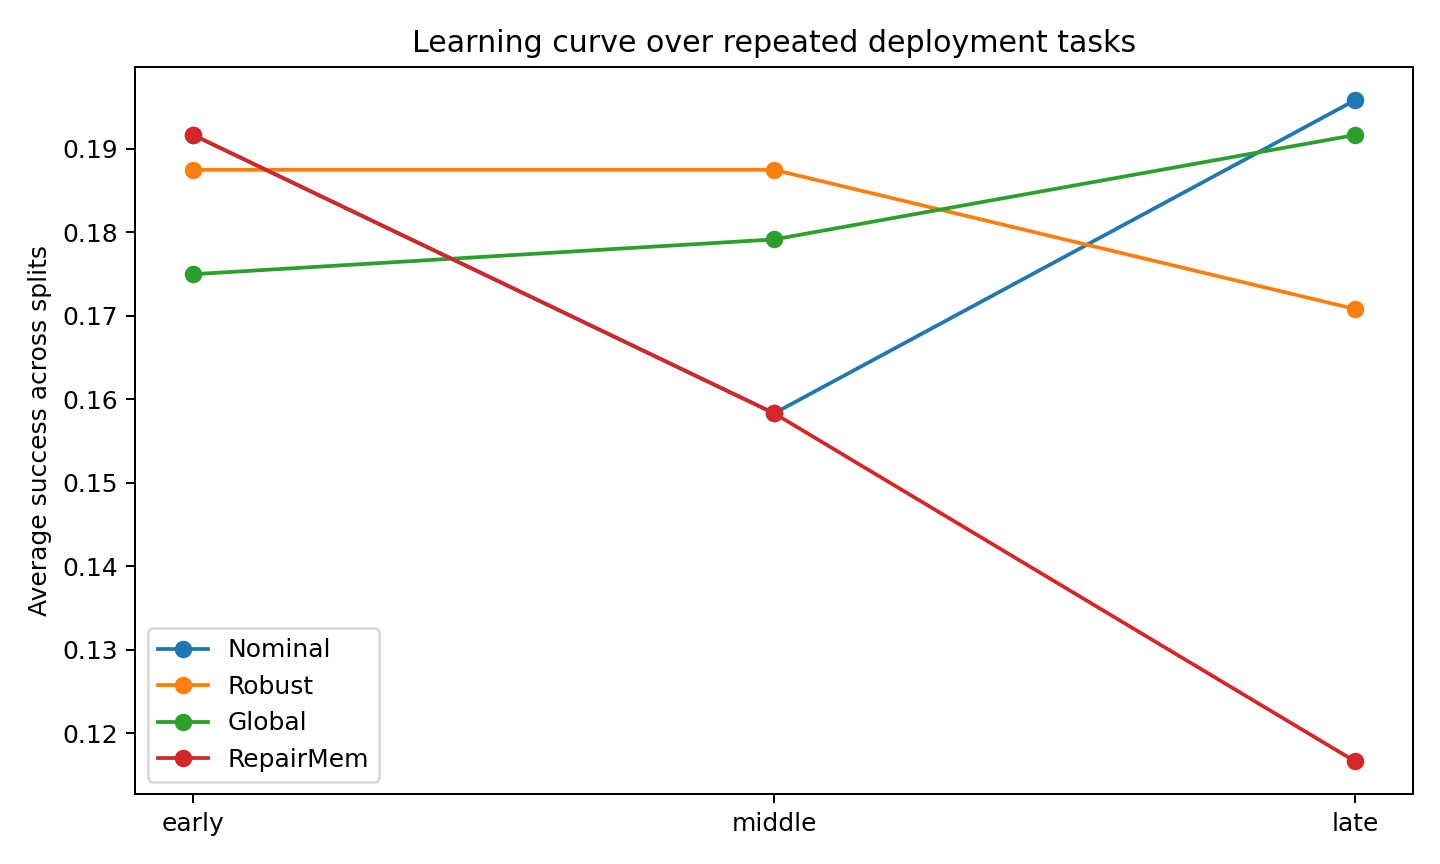
\includegraphics[width=0.85\linewidth]{../figures/repair_learning_curve.png}
\caption{Average learning curve over repeated deployment tasks. Persistent repair memory does not show the required late-stream improvement.}
\label{fig:learning}
\end{figure}

\section{Ablations}
The combined-shift ablation is also negative. Repair memory reaches $0.117 \pm 0.058$ success and 0.134 regret. Nominal/reset memory reaches $0.158 \pm 0.066$ success, while oracle reaches $0.258 \pm 0.079$ success and zero regret. Removing context or using global repair is not worse enough to isolate the proposed retrieval mechanism.

\begin{figure}[t]
\centering
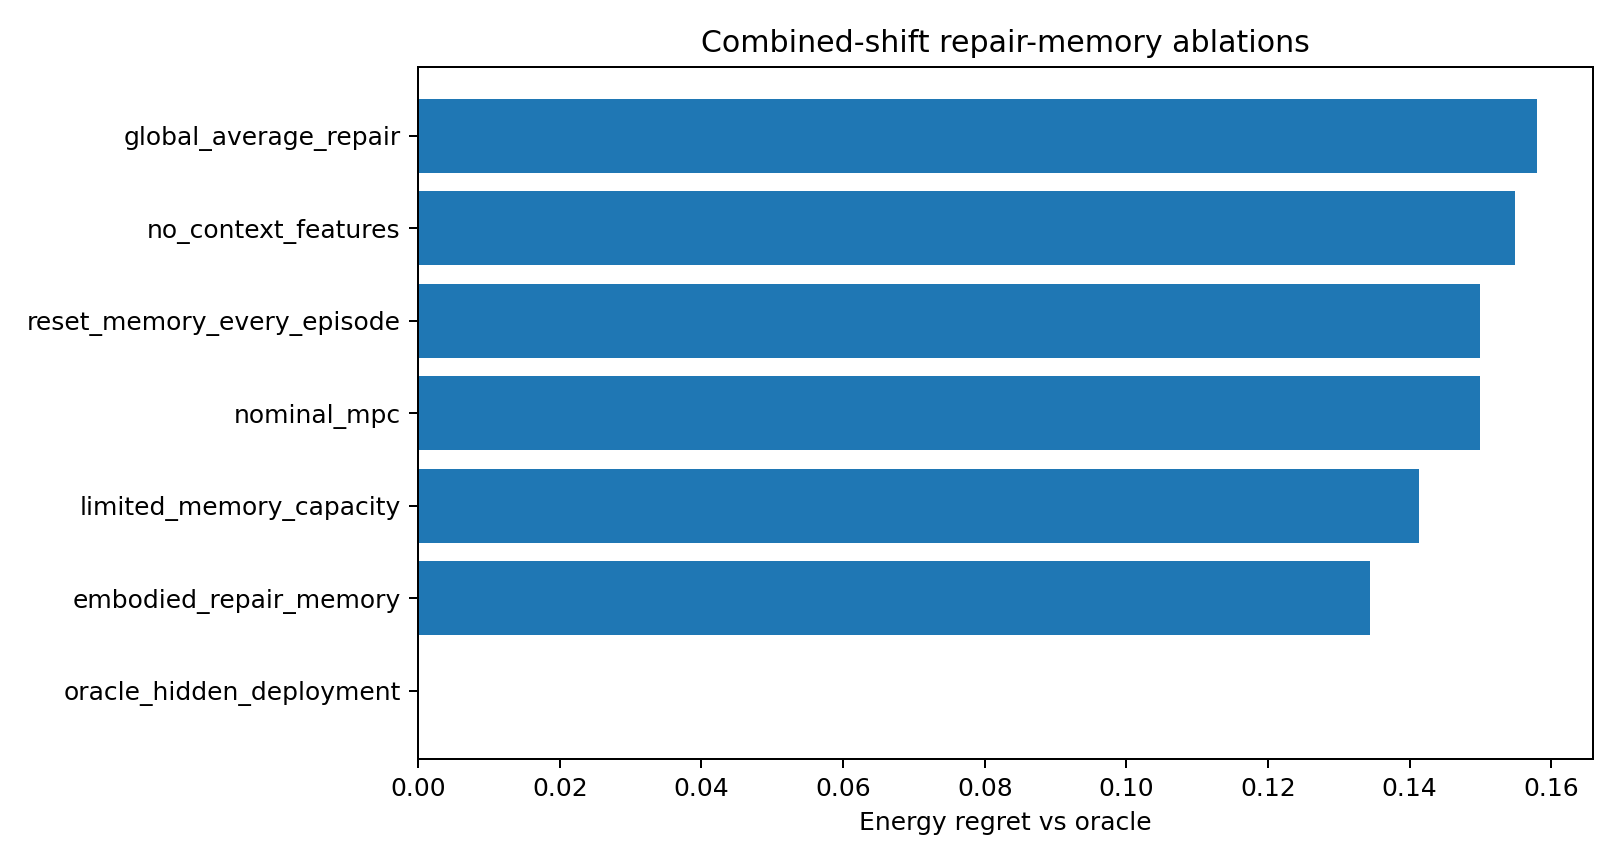
\includegraphics[width=0.85\linewidth]{../figures/repair_ablation_regret.png}
\caption{Combined-shift ablation regret. Lower is better. The proposed memory mechanism is not the best non-oracle variant.}
\label{fig:ablation}
\end{figure}

\section{Why This Kills the Current Paper}
The core claim requires reusable embodied repairs to improve later decisions under recurring physical shift. The evidence does not support that claim. The current kNN residual memory sometimes lowers regret against global repair, but it does not deliver a reliable success gain, does not improve safety enough, and does not beat robust MPC. A polished ICLR-main paper would therefore be misleading.

\section{Limitations and Revival Conditions}
This is a custom MuJoCo benchmark, not hardware or a public long-horizon manipulation benchmark. The repair model is simple kNN residual retrieval rather than a learned world-model repair module. A future revival would need a learned repair memory, stronger safety handling, and clear gains over robust MPC on CALVIN/FurnitureBench-like benchmarks or hardware.

\section{Gate Decision}
The terminal decision is \textbf{KILL\_ARCHIVE}. The v4 rebuild rescues the paper from synthetic evidence, but the real evidence kills the claim.

\end{document}
